%!TEX root = ../Thesis.tex

\section{Variational optimization}\label{sec: Variational optimization}
\Gls{VO} is an optimization technique that can be applied on almost any type of objective function including functions that are non-differentiable or discrete \cite{Staines2012}. 
This section first derives the \gls{VO} objective as a differentiable upper bound on the objective function and its gradient. 
\autoref{sec: Variational optimization: Remarks main section} then discusses \gls{VO} in relation to policy gradients, computational efficiency, dimensionality and loss surfaces and \glspl{BNN}.
The following sections present different possible choices of search distributions and derive the corresponding practical gradient estimators. Using the univariate Gaussian distribution, the intuitions of \gls{VO} are illustrated in \autoref{sec: Variational Optimization: Examples of 1D objective functions optimized with variational optimization}.


\subsection{Formal derivation}\label{sec: Formal derivation of the variational objective and gradient}
Consider the general function minimization problem $\min_\x f(\x)$ for some multivariate function $f: \mathcal{D}\rightarrow\mathcal{C}$ mapping from the domain $\mathcal{D}$ to its codomain $\mathcal{C}$ and vector input $\x\in\mathcal{D}$. The expected value of a function w.r.t. any probability distribution is guaranteed to always larger than or equal to the minimal value of the function. Equality is only achieved in the case of a constant function. Therefore, this expectation can be defined as an upper bound on the optimum of objective\footnote{This bound is obviously not true for $f(\x)$ in general but holds only at the minimum, $f(\x^*)=\min_{\x}f(\x)$.},
\begin{equation}\label{eq: Theory: Variational optimization variational upper bound}
    f(\x^*) = \min_{\x\in\mathcal{D}} f(\x) \leq \text{E}\bra{f(\x)}_{p(\x|{\thetab})} \equiv U({\thetab}) \ .
\end{equation}
Clearly, this bound can be made arbitrarily tight provided that the search distribution is flexible enough to allow for all of its probability mass to be placed in the optimum $\x^*=\arg\min_\x f(\x)$ \cite{Staines2012}.

Now, instead of minimizing $f(\x)$ w.r.t. $\x$, the upper bound $U({\thetab})$ can be optimized w.r.t. the parameters ${\thetab}$ of the search distribution $p(\x|\thetab)$. That is, the original objective function is replaced with an upper bound which is then minimized.
\begin{equation}
    f(\x^*) \leq \min_\thetab \text{E}\bra{f(\x)}_{p(\x|\thetab)} = \min_\thetab U(\thetab) \ .
\end{equation}
The gradient of the variational objective can be written as
\begin{equation}
    \nabla_{\thetab} U({\thetab}) = \nabla_{\thetab} \text{E}\bra{f(\x)}_{p(\x|\thetab)} = \nabla_{\thetab}\int_\mathcal{D} f(\x)p(\x|{\thetab}) \text{d}\x \ .
\end{equation}
By the probability identity trick and the log-derivative trick, the gradient of the upper bound can be rewritten as the expectation of a score function. The log-derivative trick is another name for the application of the chain rule to the logarithm of a function and can be written as
\begin{equation}\label{eq: Theory: Log-derivative trick for pdf}
    \nabla_{\thetab} \log p(\x|{\thetab}) = \frac{\nabla_{\thetab} p(\x|{\thetab})}{p(\x|{\thetab})} \ .
\end{equation}
The gradient of the upper bound can then be rewritten as follows
\begin{align}
\nabla_{\thetab} U({\thetab})
    &= \nabla_{\thetab}\text{E}\bra{f(\x)}_{p(\x|{\thetab})}\\
    &= \nabla_{\thetab}\int f(\x)p(\x|{\thetab}) \text{d}\x\nonumber\\
    &= \int f(\x)\nabla_{\thetab} p(\x|{\thetab}) \text{d}\x\nonumber\\
    &= \int f(\x)\nabla_{\thetab} p(\x|{\thetab})\frac{p(\x|{\thetab})}{p(\x|{\thetab})} \text{d}\x\nonumber\\
    &= \int f(\x) p(\x|{\thetab})\nabla_{\thetab}\log p(\x|{\thetab}) \text{d}\x\nonumber\\
    &= \text{E}\bra{f(\x)\nabla_{\thetab}\log p(\x|{\thetab})}_{p(\x|{\thetab})}\label{eq: Theory: Variational optimization gradient estimator general search distribution}
\end{align}
where integration and differentiation can be interchanged given the weak conditions \cite{Staines2012}:
\begin{enumerate}
    \item $f(\x)p(\x|{\thetab})$ is Lebesgue integrable and differentiable wrt. ${\thetab}$.
    \item There exists an integrable function $F: \mathcal{D}\rightarrow\mathbb{R}$ such that, for all ${\thetab}$, $\size{\nabla_{\thetab} f(\x)p(\x|\thetab)} < F(\x)$ \ .
\end{enumerate}
As noted in \cite{Staines2012}, these are often satisfied and will not be considered further here.

By evaluating the expectation with respect to $p(\x|{\thetab})$ by Monte Carlo approximation, a practical estimator becomes
\begin{align}
    \nabla_{\thetab} U({\thetab})
    &= \text{E}\bra{f(\x)\nabla_{\thetab} \log p(\x|{\thetab})}_{p(\x|{\thetab})}\nonumber\\
    &\approx \frac{1}{N}\sum_{n=1}^N f(\x_n)\nabla_{\thetab} \log p(\x_n|{\thetab}) \ .\label{eq: Theory: Variational optimization gradient estimator sampling general search distribution}
\end{align}
In an algorithmic perspective, the update to the search distribution can be computed by gradient descent
\begin{equation}
    {\thetab} \leftarrow {\thetab} - \frac{\eta}{N}\sum_{n=1}^N f(\x_n)\nabla_{\thetab} \log p(\x_n|{\thetab})
\end{equation}
for some choice of learning rate $\eta$.

This derivation allowed the transformation of the gradient of an expectation into an expectation of a score function, $\nabla_{\thetab}\log p(\x|{\thetab})$. As such, the derived estimator is a score function. Score function estimators are related to likelihood ratio methods, automated variational inference \cite{Wingate2013} and the REINFORCE rule and policy gradients \cite{Williams1992}. Additionally, it can be noted that unlike the gradient estimator derived by the Taylor expansion, the \gls{VO} gradient derived here is unbiased. Its variance is considered in \autoref{sec: Theory: Methods for variance reduction}.


\subsection{Remarks on variational optimization}\label{sec: Variational optimization: Remarks main section}
Before proceeding with different search distributions, a few remarks will be made about \gls{VO} in relation to \glspl{BNN}, policy gradients, computational efficiency, dimensionality and loss surfaces.

\subsubsection{Relation to Bayesian neural networks}
A \gls{BNN} is a combination of a probabilistic graphical model and a neural network. The result of training is not a point estimate of the weights but a full posterior distribution over the weights \cite{Goodfellow2016}. With \gls{VO}, a search distribution over potential weights is maintained and adjusted during training in order to minimize the \gls{VO} upper bound on the objective. The result is in fact a distribution over the weights however, using e.g. a Gaussian search distribution, the variance is potentially driven to zero, effectively yielding a point estimate as in the standard maximum likelihood approach. Additionally, the variance of the search distribution does not directly reflect uncertainty in the parameter estimates but instead the degree of smoothing applied to the potentially non-smooth objective at each iteration.

\subsubsection{Comparison to policy gradient methods}
The policy gradients approach to \gls{RL} can be formulated as seeking to maximize some reward $R$ which depends on a sequence of actions $\a=\cbra{a_1,\dots,a_T}$ that are in turn determined by a policy network parameterized by a number of parameters $\mub$. The function to be optimized is then $f(\mub) = R(\a(\mub))$.
The possibility of discrete actions and deterministic policy allows $f(\mub)$ to be a non-smooth function. This, and the lack of knowledge about the environment state transition function makes direct application of gradient based optimization of the policy impossible \cite{Salimans2017}.

To obtain gradient estimates, noise must be added to the objective and this is where policy gradients and \gls{VO} differ.
As described, \gls{VO} adds noise in the parameter space and then picks the most probable action at each iteration. This gives the gradient in \eqref{eq: Theory: Variational optimization gradient estimator sampling general search distribution}. As will be shown later (\autoref{sec: Theory: Methods for variance reduction}), the variance of the \gls{VO} gradient can be written as
\begin{equation}\label{eq: Theory: VO gradient variance}
    \text{Var}\bra{\nabla_\thetab U(\thetab)} = \frac{1}{N}\text{Var}\bra{R(\a(\x))\nabla_\thetab\log p(\x|\thetab)}
\end{equation}
where $N$ is the number of perturbations used for the Monte Carlo estimation and $\x$ is a perturbation of the parameters, $\x=\mub+\epsilonb$. The policy parameters $\mub$ are included in the search distribution parameter vector $\thetab$ which can also include other parameters relevant for the distribution. 

Policy gradients on the other hand adds the noise in the action space by sampling the action to take at each iteration from a categorical distribution estimated by the policy network. For a discrete action space, the policy gradients objective can be written as \cite{Salimans2017}
\begin{equation}
    \nabla_\mub f(\mub, \epsilon) = \text{E}_\epsilon\bra{R(\a(\mub, \epsilon))\nabla_\mub\log p(\a(\mub, \epsilon)|\mub)} \ .
\end{equation}
where $\epsilon$ is the random variable used for sampling. When computing this gradient by Monte Carlo estimation, its variance becomes \cite{Salimans2017}
\begin{equation}\label{eq: Theory: Policy gradients gradient variance}
    \text{Var}\bra{\nabla_\mub f(\mub, \epsilon)} \approx \text{Var}\bra{R(\a(\mub, \epsilon))\nabla_\mub\log p(\a(\mub,\epsilon)|\mub)} \ .
\end{equation}
This follows from calculations similar to those that will be made in \autoref{sec: Theory: Methods for variance reduction} which considers variance reduction methods for \gls{VO}.

Now, the variance of the \gls{VO} and policy gradients in \eqref{eq: Theory: VO gradient variance} and \eqref{eq: Theory: Policy gradients gradient variance} can be compared. 
If the total reward is only weakly correlated with each action in $\a$, then 
\begin{align}
    \text{Var}\bra{\nabla_\thetab U(\thetab)} &\approx \frac{1}{N}\text{Var}\bra{R(\a(\x))}\text{Var}\bra{\nabla_\thetab\log p(\x|\thetab)}\\
    \text{Var}\bra{\nabla_\mub f(\mub, \epsilon)} &\approx \text{Var}\bra{R(\a(\mub, \epsilon))}\text{Var}\bra{\nabla_\mub\log p(\a(\mub,\epsilon)|\mub)} \ .
\end{align}
This is often the case in a difficult \gls{RL} problem.
If the amount of exploration is similar in the two methods then $\text{Var}\bra{R(\a(\mub, \epsilon))}\sim\text{Var}\bra{R(\a(\x))}$. The difference is then in last term. 
For policy gradients, $\nabla_\mub\log p(\a(\mub,\epsilon)|\mub)$ is a sum of uncorrelated terms of each action taken and thus its variance increases linearly with the episode horizon, $T$. The \gls{VO} variance does not depend on $T$ but instead decreases with increasing number of evaluated perturbations. When effects are long-lasting, the conventional way to reduce the policy gradients variance by discounting rewards can introduce bias in the gradient estimate. In this case, \gls{VO} may provide a better gradient estimate. 

Another approach to variance reduction in policy gradients is through a hybridization with value function approximations called actor-critic policy gradients. Here, the action-value function $Q(\s,\a)$ is approximated which measures the value (or quality) of taking action $\a$ in state $\s$ and replaces the reward returned by the environment. This reduces variance but introduces bias by approximating the gradient. In order to further reduce variance, a baseline can be substracted from $Q(\s,\a)$. A good baseline is the value function $V(\s)$ which gives the value of any state and must also be estimated. The result is the advantage function $A(\s,\a)=Q(\s,\a)-V(\s)$ \cite{Arulkumaran2017}. In \gls{VO} a similar approach exists under the name of fitness baselines which also subtract a constant term from the objective function in order to reduce variance \cite{Yi2009}. This approach does not require the approximation of one or two additional value functions but instead relies on the search distribution, its \gls{FIM} and the objective function evaluations already made.


\subsubsection{Computational considerations}
The computation of the gradient of the \gls{VO} objective by Monte Carlo approximation is easily parallelized as each function evaluation is independent of any other evaluations. If the evaluation of each $f(\x_n)\nabla_{\thetab} \log p(\x_n|{\thetab}))$ is time consuming or $N$ is very large, significant speed up can be expected by distributing these computations among many \glspl{CPU}. Furthermore, the search points $\x_n$ are uniquely defined by their probability distribution and the random seed that was used to sample them. That is, all information required to request and return a term of the gradient estimator, is the random seed used to sample $\x_n$ and the function value $f(\x_n)$. This allows for low-bandwidth communication between individual machines, in turn making viable the distribution of the computation to a large number of \glspl{CPU} on many distinct machines that do not share memory. Pseudocode for this algorithm can be seen in \autoref{alg: Canonical variational optimization}. 

\begin{algorithm}[tbp!]
	\caption{Parallelized Variational Optimization. Adapted from \cite{Wierstra2008} \label{alg: Canonical variational optimization}}
	\begin{algorithmic}[1]
		\Require{Learning rate $\eta$, search distribution $p(\x|\thetab)$, objective function $f(\x)$}
		\Initialize{$N$ workers with known random seeds}
		\Repeat
			\For{each \gls{CPU} $i=1,\dots,N$} \Comment{Parallelizable}
			    \State Draw random seed $s_i$
				\State Sample $\x_i\sim p(\x|\thetab)$
				\State Evaluate fitness $f(\x_i)$
			\EndFor
			\State Share $N$ scalar fitnesses, $f(\x_i)$ and seeds, $s_i$, between all \glspl{CPU}.
			\For{each worker $i=1,\dots,N$} \Comment{Parallelizable}
				\State Reconstruct all perturbations $\x_j$ for $j=1,\dots,N$ using known random seeds.
				\State Compute search distribution and upper bound gradient
				$$\nabla_\thetab U(\thetab) = \frac{1}{N}\sum_{n=1}^N f(\x_i) \nabla_\thetab\log p(\x_i|\thetab)$$
				\State Update search distribution parameters 
				$$\thetab \gets \thetab - \eta\nabla_\thetab U(\thetab)$$
			\EndFor
		\Until{stopping criteria met}
	\end{algorithmic}
\end{algorithm}


\subsubsection{Dimensionality and loss surfaces}\label{sec: Theory: Variational optimization: Remarks on dimensionality}
There is a classical distinction to be made on the ratio of the dimensionality of the search space, $d$, and the number of perturbations on which the gradient estimate is based, $N$. There are two cases: When $d<N$ the sampled perturbations will likely span the entire search space. However, when $d>N$ then, even though each of the perturbations add noise to every dimension of the search space, they only span a subspace of the search space. Using standard \gls{VO}, this subspace will be selected implicitly at random at each iteration by the sampling of the perturbations.

A note can be made on the intrinsic dimension of objective landscapes encountered in different problems. Recently \cite{Li2018a} it was shown that many problems have an intrinsic dimension much lower than the number of parameters in the \glspl{NN} typically trained for solving them. 
By training models in a small random subspace of their parameter spaces and monitoring solutions while iteratively increasing the subspace size, the authors define the intrinsic problem dimension to be that where the first good solutions arise. 
In \gls{VO}, the training procedure is similar to this, but the subspace of the parameter space is selected implicitly at random at each iteration instead of being fixed throughout training. In fact, in high-dimensional search spaces, each of the perturbations sampled at each iteration will likely span a unique subspace such that search is actually performed in multiple non-overlapping subspaces.

A fair amount of research has focused on describing the high-dimensional loss surfaces of neural networks.
In \cite{Dauphin2014}, it was shown that local minima are exponentially less frequent in high dimensional non-convex optimization than are saddle points.
\cite{Goodfellow2015} showed that for \glspl{NN} there exists a linear subspace in which training can proceed by descending along a monotonically decreasing path with no barriers, in line with the rarity of local minima. These properties affect \gls{VO} and are discussed further in \autoref{sec: Experimental work: Effect of adapting the variance}.

Finally, it can be imagined that the gradient estimate of one iteration may be able to benefit from information from the previous iteration(s). A simple way to exploit this is by adding momentum to the gradient. Another rendering of this information could be by explicitly computing promising dimensions for search. Ideas related to this are investigated further in \autoref{sec: Theory: Importance mixing} and \autoref{sec: Theory: Adaptation sampling}.




% \newline
% \newline
% In the following sections, the \gls{VO} gradient is derived for specific choices of search distribution.



\subsection{Search distributions}
When \gls{VO} is applied to optimization of \glspl{NN}, $\x$ represents the perturbed parameters of the model while the search distribution defines how these parameters are sampled. When training \glspl{NN} with Gaussian search distributions, the mean vector $\mub$ parameterizes the best current estimate of the network parameters and constitutes what is here called the unperturbed model. The covariance matrix defines how and how much the sampled parameters $\x$ deviate from $\mub$.

%Similarly to what was done for the Taylor series estimator, it is convenient to write the sampled parameters as $\x = \mub + \epsilonb$ where $\epsilonb$ is some perturbation that can be sampled by the reparameterization trick.

This section first derives a univariate Gaussian estimator in order to exemplify the intuitions of \gls{VO}. Then it derives the isotropic and separable Gaussian \gls{VO} gradient estimators which are central for \gls{VO} and are used in the experimental section. 
%in one-dimensional function optimization. 
The multivariate Gaussian is also treated and a potential approach for making its covariance matrix computationally feasible using a low-rank approximation is presented.

\subsubsection{Univariate Gaussian search distribution}\label{sec: Theory: Variational optimization: Univariate Gaussian search distribution}
Let $p(\x|\thetab) = \mathcal{N}(x|\mu,\sigma^2)$ be a univariate Gaussian distribution
\begin{equation}
    \mathcal{N}(x|\mu,\sigma^2) = \frac{1}{\sqrt{2\pi\sigma^2}}\exp\left(-\frac{1}{\sigma^2}(x-\mu)^2\right)
\end{equation}
where $\thetab=\bmat{\mu,\sigma^2}\transpose$ so $U(\thetab)=U(\mu,\sigma^2)$. Let $x = \mu + \sigma\epsilon$ with $\epsilon\sim\mathcal{N}(0,1)$. Then by \eqref{eq: Theory: Variational optimization variational upper bound}
\begin{equation}
    U(\mu,\sigma^2) = \text{E}\bra{f(x)}_{\mathcal{N}(x|{\mu,\sigma^2})}  = \text{E}\bra{f(\mu + \sigma\epsilon)}_{\mathcal{N}(\epsilon|{0,1})} \ .
\end{equation}
The logarithm of the univariate Gaussian is given by
\begin{equation}
    \log\mathcal{N}(x|\mu,\sigma^2) = -\frac{1}{2}\log 2\pi - \frac{1}{2}\log\sigma^2 - \frac{1}{2\sigma^2}(x-\mu)^2 \ ,
\end{equation}
%and
%\begin{align}
%    \pderiv{}{\mu} U(\mu,\sigma^2)
%    &= \text{E}\bra{f(x)\pderiv{}{\mu}\log \mathcal{N}(x|{\mu,\sigma^2})}_{\mathcal{N}(x|{\mu,\sigma^2})}\nonumber\\
%    &= \text{E}\bra{f(\mu+\sigma\epsilon)\pderiv{}{\mu}\log\mathcal{N}(x|{\mu,\sigma^2})}_{\mathcal{N}(\epsilon|{0,1})}
%\end{align}
%which holds similarly for the variance. 
with derivatives computed as
\begin{equation}
    \begin{aligned}
        \pderiv{}{\mu}\log\mathcal{N}(x|\mu,\sigma^2) &= \frac{1}{\sigma^2}(x-\mu) = \frac{1}{\sigma}\epsilon\\
        \pderiv{}{\sigma^2}\log\mathcal{N}(x|\mu,\sigma^2) &= -\frac{1}{2\sigma^2} + \frac{1}{2\sigma^4}(x-\mu)^2  = \frac{1}{2\sigma^2}\pa{\epsilon^2-1} \ . % = \frac{1}{2\sigma^2}\left(\frac{1}{\sigma^2}(x-\mu)^2 - 1\right).
    \end{aligned}\label{eq: Theory: Variational optimization univariate gaussian search gradients}
\end{equation}
The gradient of the upper bound with respect to the parameters of the search distribution is then
\begin{equation}
    \begin{aligned}
        \pderiv{}{\mu}U(\mu,\sigma^2) &= \frac{1}{\sigma}\text{E}\bra{f(\mu + \sigma\epsilon)\epsilon} \approx \frac{1}{N\sigma}\sum_{n=1}^N f(\mu+\sigma\epsilon_n)\epsilon_n\\
        \pderiv{}{\sigma^2}U(\mu,\sigma^2) &= \frac{1}{2\sigma^2}\text{E}\bra{f(\mu + \sigma\epsilon)\left(\epsilon^2-1\right)} \approx \frac{1}{2N\sigma^2}\sum_{n=1}^N f(\mu + \sigma\epsilon_n)\left(\epsilon_n^2-1\right)\\
    \end{aligned}\label{eq: Theory: Variational optimization univariate gaussian gradient estimators}
\end{equation}
where it has been used that $\nabla_{\thetab} U({\thetab}) = \text{E}\bra{f(\x)\nabla_{\thetab} \log p(\x|{\thetab})}_{p(\x|{\thetab})}$ as derived in \eqref{eq: Theory: Variational optimization gradient estimator general search distribution} with $\thetab=\bmat{\mu & \sigma^2}\transpose$.

It can be noted that the derived first order derivative of the upper bound w.r.t. $\mu$ in \eqref{eq: Theory: Variational optimization univariate gaussian gradient estimators} is in fact identical to the estimator for the first order derivative of the objective function as derived by Taylor expansion in \eqref{eq: Theory: Taylor: Univariate gradient estimator from standard Gaussian}. This establishes a clear connection between the gradient estimate of \cite{Salimans2017} and \gls{VO}: The estimator in \cite{Salimans2017} can be seen as a special case of \gls{VO} using a Gaussian search distribution and a fixed variance.

The Taylor estimator in \eqref{eq: Theory: Taylor: Univariate gradient estimator from standard Gaussian} is biased due to the negligence of the remainder term but the estimator derived here is in fact unbiased. Since the two estimators are equal it must be concluded that the remainder of Taylor expansion estimator has an expected value of zero.

During optimization of the search distribution parameters, it must be ensured that $\sigma>0$ at every iteration.
A simple way to achieve this is by an exponential reparameterization of the variance. Let
\begin{equation}
    \sigma^2 = e^{\beta} \ .
\end{equation}
Since $e^{\beta}>0\;\forall\beta$ then by optimizing $\beta$ rather than $\sigma$ the constraint $\sigma>0$ is guaranteed to be satisfied. With this parameterization
\begin{equation}
    \log\mathcal{N}(x|\mu,\beta)= -\frac{1}{2}\log 2\pi - \frac{1}{2}\beta - \frac{1}{2}e^{-\beta}(x-\mu)^2,
\end{equation}
such that
\begin{equation}
    \begin{aligned}
        \pderiv{}{\mu}\log\mathcal{N}(x|\mu,\beta) &= e^{-\beta}(x-\mu) = e^{-\frac{1}{2}\beta}\epsilon\\
        \pderiv{}{\beta}\log\mathcal{N}(x|\mu,\beta) &= -\frac{1}{2} + \frac{1}{2}e^{-\beta}(x-\mu)^2  = \frac{1}{2}\pa{\epsilon^2-1} % = \frac{1}{2\sigma^2}\left(\frac{1}{\sigma^2}(x-\mu)^2 - 1\right).
    \end{aligned}\label{eq: Theory: Variational optimization univariate gaussian search gradients (exponential parameterization)}
\end{equation}
and
\begin{equation}
    \begin{aligned}
        \pderiv{}{\mu}U(\mu,\beta) &= \frac{1}{\sigma}\text{E}\bra{f\pa{\mu + e^{\frac{1}{2}\beta}\epsilon}\epsilon} \approx \frac{e^{-\beta}}{N}\sum_{n=1}^N f\pa{\mu+e^{\frac{1}{2}\beta}\epsilon_n}\epsilon_n\\
        \pderiv{}{\beta}U(\mu,\beta) &= \frac{1}{2}\text{E}\bra{f\pa{\mu + e^{\frac{1}{2}\beta}\epsilon}\left(\epsilon^2-1\right)} \approx \frac{1}{2N}\sum_{n=1}^N f\pa{\mu + e^{\frac{1}{2}\beta}\epsilon_n}\left(\epsilon_n^2-1\right) \ .
    \end{aligned}
    \label{eq: Theory: Variational optimization univariate gaussian gradient estimators (exponential parameterization)}
\end{equation}
This is essentially the same result for $\mu$ as before. The derivative w.r.t. $\beta$ however only depends on $\beta$ through the function evaluations and not in the factor in front of the sum, as was the case for the derivative w.r.t. $\sigma^2$. This type of reparameterization can be directly applied for all Gaussians with diagonal covariance. This is done throughout the thesis.


\subsubsection{Examples for the univariate Gaussian}\label{sec: Variational Optimization: Examples of 1D objective functions optimized with variational optimization}
% We need the sinc function for this section
\providecommand{\sinc}{{\text{sinc}}}
For the univariate Gaussian distribution considered here, it is possible to visualize the intuition of \gls{VO}. The effect of applying \gls{VO} with a univariate Gaussian to a univariate objective function is to turn the one-dimensional optimization problem $\min_x f(x)$ into a two-dimensional one, $\min_{\{\mu,\sigma^2\}} U(\mu,\sigma^2)$. 

Specifically, consider the negative $\sinc$ function, defined as $\sinc(x) = \sin(\pi x)/\pi x$ seen in \autoref{fig: Theory: var-opt-intu-sinc-function}. If one were to optimize the $\sinc$ function using gradient descent, the resulting minimum would be highly dependent on the choice of the initial point with the algorithm converging to the global minimum only for initial points between about $\pm 1.43$. 
%
%
\begin{figure}[tbp!]
    \begin{subfigure}[b]{0.49\textwidth}
        \centering
        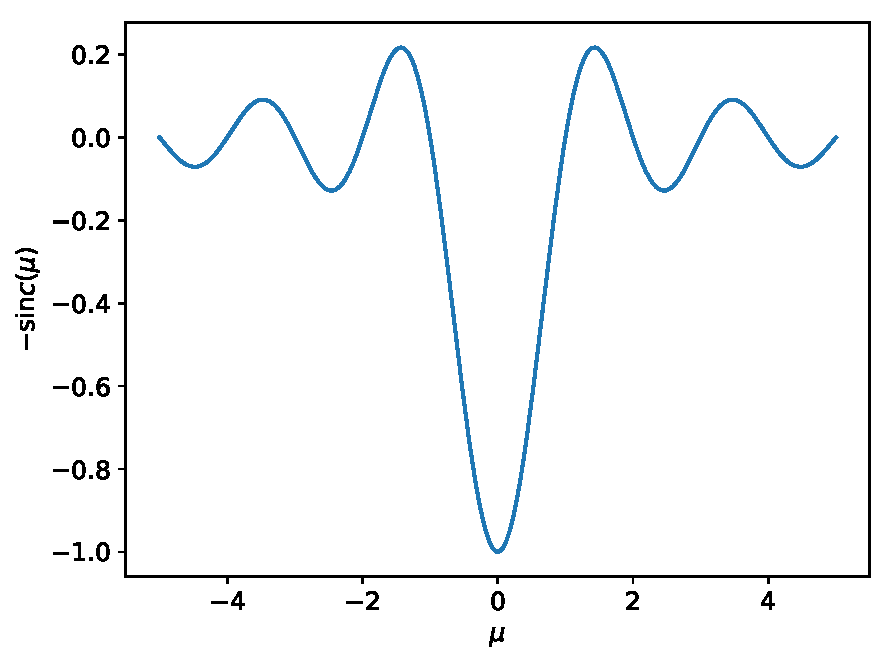
\includegraphics[height=5.7cm]{graphics/var-opt-intu/variational-optimization-function-sinc.pdf}
        \caption{}
        \label{fig: Theory: var-opt-intu-sinc-function}
    \end{subfigure}
    \hfill
    \begin{subfigure}[b]{0.49\textwidth}
        \centering
        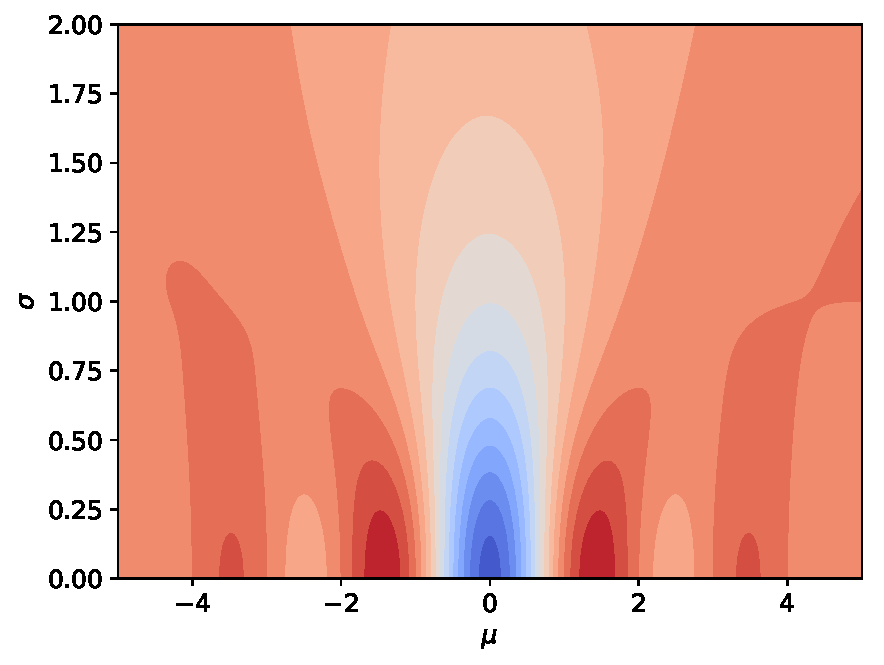
\includegraphics[height=5.7cm]{graphics/var-opt-intu/variational-optimization-contour-sinc.pdf}
        \caption{}
        \label{fig: Theory: var-opt-intu-sinc-contour}
    \end{subfigure}
    \caption{\subref{fig: Theory: var-opt-intu-sinc-function} The negative $\sinc$ function. \subref{fig: Theory: var-opt-intu-sinc-contour} The contours of the Gaussian \gls{VO} objective for the $\sinc$ function for different values of $\mu$ and $\sigma$. Here, the \gls{VO} objective is a two-dimensional upper bounding version of the $\sinc$ function. It tends to a constant for $\sigma\rightarrow\infty$ and the $\sinc$ function for $\sigma\rightarrow0$. The \gls{VO} objective is slightly asymmetrical due to being computed by sampling. Red denotes high values, blue denotes low values and the darker the colour, the higher the absolute value. Actual values are omitted for simplicity. Figures inspired by \cite{Huszar2017}.}
    \label{fig: Theory: var-opt-intu-sinc}
\end{figure}
%
%
The Gaussian \gls{VO} objective function corresponding to the $\sinc$ is visualized in \autoref{fig: Theory: var-opt-intu-sinc-contour} for different values of the search distribution variables $\mu$ and $\sigma^2$. Note especially that optimization is now over the parameters of the search distribution. The global minimum is at $\mu=0$ for any value of $\sigma$. The new objective still has the exact form of the original for $\sigma=0$ and as such still has challenging local minima. However, in this specific case, minimizing the \gls{VO} objective with a fixed value of $\sigma$ of about 1 or larger would uniformly result in approximate\footnote{The convergence will only be to an approximation of the minimum when $\sigma$ is held fixed. This is discussed further in \autoref{sec: Natural Gradient}} convergence on the global minimum regardless of initial point.
Additionally, notice that around the global minimum, $\sinc$ is convex which is also true for the \gls{VO} objective. In fact, for any expectation affine search distribution, which includes Gaussians, if the original objective function is convex then so is the the variational upper bound \cite{Staines2012}.

A quantized version of the $\sinc$ function is seen in \autoref{fig: Theory: var-opt-intu-sinc-quantized-function}. Although this function is non-differentiable, the \gls{VO} bound is still differentiable for any non-zero variance as can be seen in \autoref{fig: Theory: var-opt-intu-sinc-quantized-contour}. As the search distribution variance approaches zero, the \gls{VO} objective tends towards the original objective and non-differentiability. Letting $\sigma\rightarrow\infty$ results in the \gls{VO} objective approaching a constant yielding zero gradient everywhere.
\begin{figure}[tbp!]
    \begin{subfigure}[b]{0.49\textwidth}
        \centering
        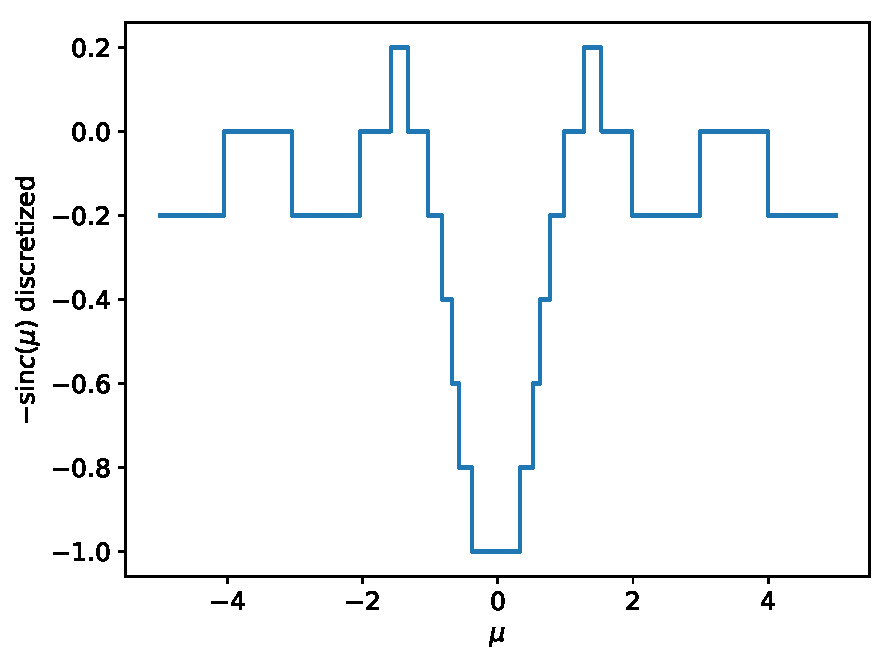
\includegraphics[height=5.7cm]{graphics/var-opt-intu/variational-optimization-function-sinc_quantized.pdf}
        \caption{}
        \label{fig: Theory: var-opt-intu-sinc-quantized-function}
    \end{subfigure}
    \hfill
    \begin{subfigure}[b]{0.49\textwidth}
        \centering
        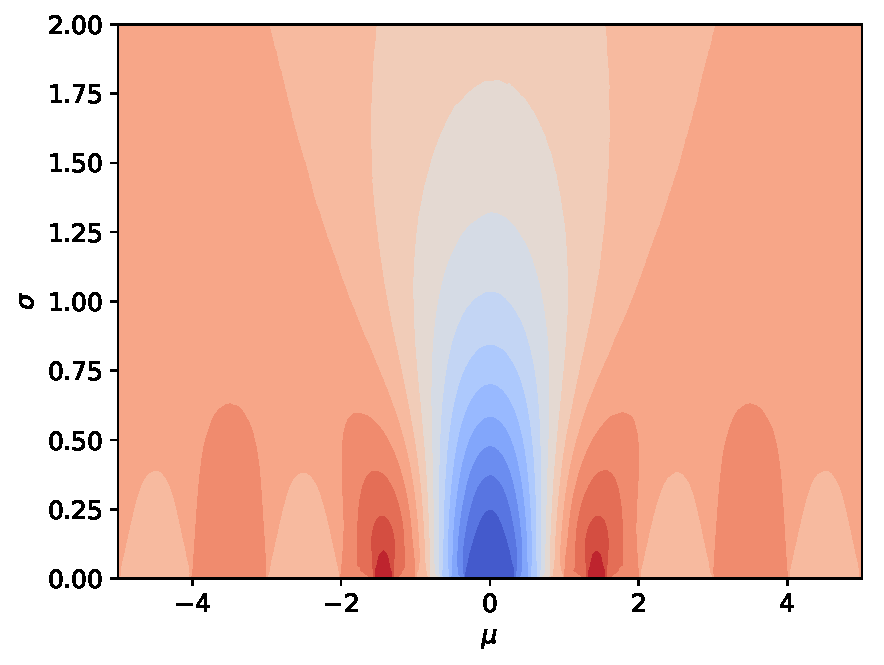
\includegraphics[height=5.7cm]{graphics/var-opt-intu/variational-optimization-contour-sinc_quantized.pdf}
        \caption{}
        \label{fig: Theory: var-opt-intu-sinc-quantized-contour}
    \end{subfigure}
    \caption{\subref{fig: Theory: var-opt-intu-sinc-quantized-function} A quantized version of the $\sinc$ function shown in \autoref{fig: Theory: var-opt-intu-sinc-function}. \subref{fig: Theory: var-opt-intu-sinc-quantized-contour} The contours of the corresponding Gaussian \gls{VO} objective for different values of $\mu$ and $\sigma$. The \gls{VO} objective is a smoothed version of the original nondifferentiable objective tending towards a constant for $\sigma\rightarrow\infty$ and non-differentiability for $\sigma\rightarrow0$. Figures inspired by \cite{Huszar2017}.}
    \label{fig: Theory: var-opt-intu-sinc-quantized}
\end{figure}


A final point should be made about the smoothing of the original objective function done by \gls{VO}. \autoref{fig: Theory: var-opt-intu-narrow-vs-wide-function} shows a function that has a wide local minimum and a narrow global minimum. As seen in \autoref{fig: Theory: var-opt-intu-narrow-vs-wide-contour}, the \gls{VO} objective has a clear preference toward the wide local minimum. The reason for this preference is that the expectation is computed based on a specific value of the variance. The larger the variance, the wider is the range of values on which the function is evaluated and the expectation computed. For large values of $\sigma$, narrow minima are simply averaged out due to the high function values for most sampled points. Thus, Gaussian \gls{VO} has a bias towards minima with low curvature compared to minima with high curvature. This bias is similarly present for other search distributions. 
In relation to this, it is interesting to note that the local structure of the minima of \gls{NN} loss surfaces has been shown to have strong connections to the ability of the resulting network to generalize well. Flatter minima have been claimed to yield better generalization than sharp although the way to define flatness in high dimensional geometries remains somewhat intangible \cite{Garipov2018}.
%
%
\begin{figure}[tbp!]
    \begin{subfigure}[b]{0.49\textwidth}
        \centering
        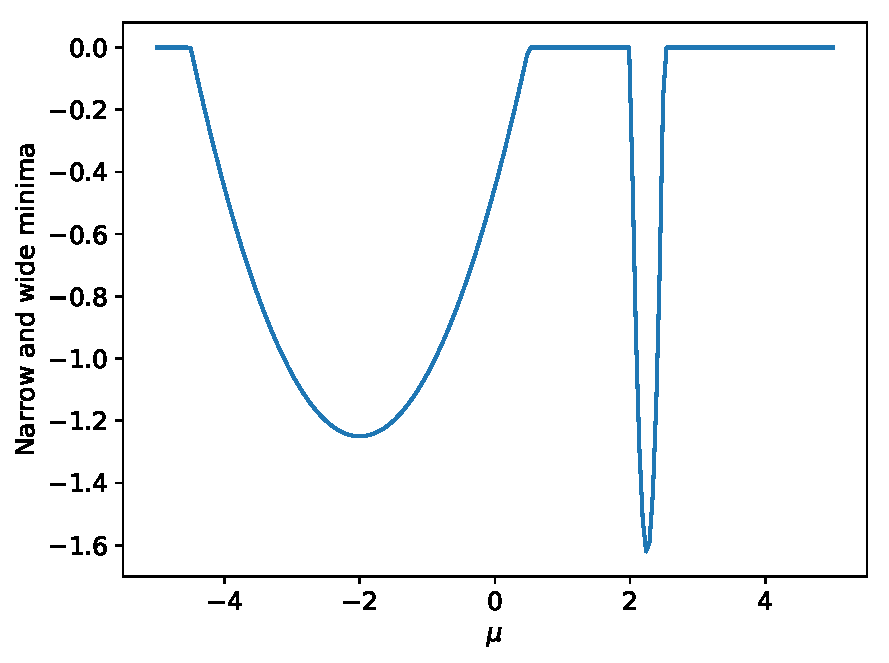
\includegraphics[height=5.7cm]{graphics/var-opt-intu/variational-optimization-function-narrow_vs_wide.pdf}
        \caption{}
        \label{fig: Theory: var-opt-intu-narrow-vs-wide-function}
    \end{subfigure}
    \hfill
    \begin{subfigure}[b]{0.49\textwidth}
        \centering
        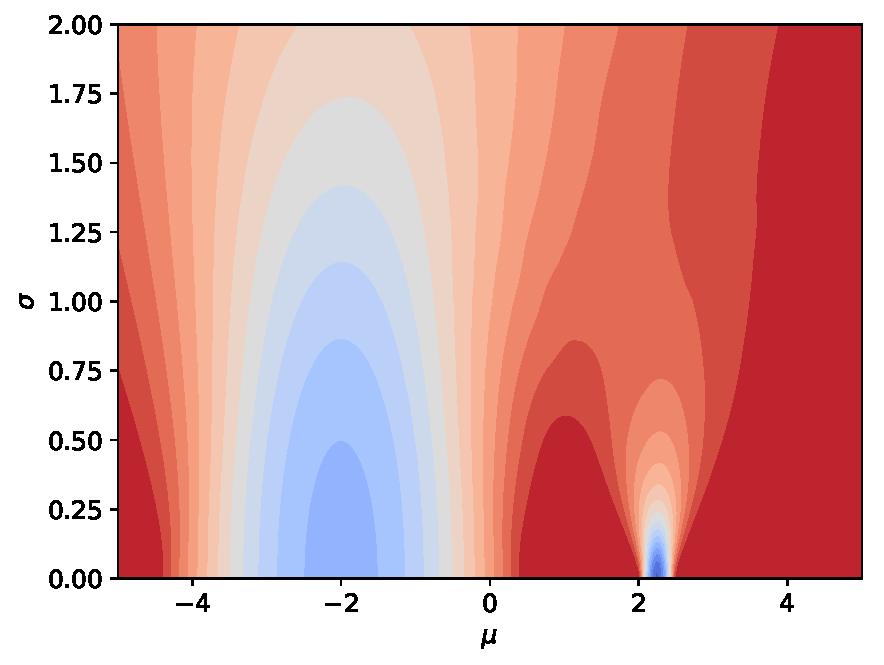
\includegraphics[height=5.7cm]{graphics/var-opt-intu/variational-optimization-contour-narrow_vs_wide.pdf}
        \caption{}
        \label{fig: Theory: var-opt-intu-narrow-vs-wide-contour}
    \end{subfigure}
    \caption{\subref{fig: Theory: var-opt-intu-narrow-vs-wide-function} A function with a low curvature local minimum and a high curvature global minimum. \subref{fig: Theory: var-opt-intu-narrow-vs-wide-contour} The contours of the corresponding Gaussian \gls{VO} objective. The Gaussian \gls{VO} objective has a different global minimum than the original function for almost all values of $\sigma>0$. This illustrates the tendency of \gls{VO} to prefer low curvature minima over high curvature minima if situated near each other. Figures inspired by \cite{Huszar2017}.}
    \label{fig: Theory: var-opt-intu-narrow-vs-wide}
\end{figure}
%
%
\iffalse
\begin{equation}
    \nabla_{\thetab} U({\thetab}) = \text{E}\bra{f(\x)\nabla_{\thetab} \log p(\x|{\thetab})}_{p(\x|{\thetab})}\nonumber\\
\end{equation}


\begin{equation}
    \mathcal{N}(x|\mu,\sigma^2) = \mathcal{N}(\epsilon+\mu|\mu,\sigma^2) = \frac{1}{\sqrt{2\pi\sigma^2}}\exp\left(-\frac{1}{\sigma^2}\epsilon^2\right) = \mathcal{N}(\epsilon|0,\sigma^2)
\end{equation}


Now
\begin{equation}
    \nabla_{\thetab} \log p(x|{\thetab}) = \bmat{\frac{1}{\sigma^2}(x-\mu) \\ -\frac{1}{2\sigma^2} + \frac{1}{4\sigma^4}(x-\mu)^2}
\end{equation}
and
\begin{equation}
    \nabla_{\thetab} U({\thetab}) = \bmat{\pderiv{}{\mu} U(\mu,\sigma^2) \\ \pderiv{}{\sigma^2} U(\mu,\sigma^2)}
\end{equation}

Inserting this in \eqref{eq: Theory: Variational optimization gradient estimator general search distribution} and \eqref{eq: Theory: Variational optimization gradient estimator sampling general search distribution} yields a gradient estimator for optimization of general univariate objective functions
\begin{equation}
    \nabla_{\thetab} U({\thetab}) = \text{E}_{p(\x|{\thetab})}\bra{f(\x)\nabla_{\thetab} \log p(\x|{\thetab})} = \bmat{\pderiv{}{\mu} U(\mu,\sigma^2) \\ \pderiv{}{\sigma^2} U(\mu,\sigma^2)} = \bmat{ \text{E}\left[f(x)\pderiv{}{\mu}\log\mathcal{N}(x|\mu,\sigma^2)\right] \\ \text{E}\left[f(x)\pderiv{}{\sigma^2}\log\mathcal{N}(x|\mu,\sigma^2)\right]}
    %U(\mu,\sigma^2)}\\
    %\nabla_{\thetab}\text{E}_{p(\x|{\thetab})}\bra{f(\x)}\nonumber\\
%&= \text{E}_{p(\x|{\thetab})}\bra{f(\x)\nabla_{\thetab} \log p(\x|{\thetab})}\nonumber\\
%&\approx \frac{1}{N}\sum_{n=1}^N f(\x_n)\nabla_{\thetab} \log p(\x_n|{\thetab}))
\end{equation}
\fi




%\subsubsection{The non-general equality of the Taylor series gradients and the variational upper bound gradients}
\subsubsection{The difference between the VO and Taylor series gradients}
Following the observation that the Taylor gradient and the \gls{VO} gradient are equivalent for a Gaussian perturbation/search distribution, it should be noted the two approaches are not in general equivalent for different choices of search distributions. As an example, take the Laplace distribution,
\begin{equation}
    p(x|\mu,b) = \frac{1}{2b}\exp\pa{-\frac{\size{x-\mu}}{b}} = \frac{1}{\sqrt{2}\sigma}\exp\pa{-\frac{\sqrt{2}}{\sigma}\size{x-\mu}}
\end{equation}
with mean $\mu$ and variance $\sigma=\sqrt{2}b$. The first three moments of the Laplace distribution are needed for the Taylor gradient estimator and can be computed as follows. Let $\epsilon = x-\mu$ from which it follows that $d\epsilon = dx$. The first moment is
\begin{align}
    \text{E}\bra{x}
    &= \text{E}\bra{\epsilon}+\mu\nonumber\\
    &= \frac{1}{2b}\int_{-\infty}^{\infty} \epsilon \exp\pa{-\frac{\size{\epsilon}}{b}}\;\text{d}\epsilon + \mu\nonumber\\
    &= \frac{1}{2b}\pa{\int_{-\infty}^{0} \epsilon \exp\pa{\frac{\epsilon}{b}}\;\text{d}\epsilon + \int_{0}^{\infty} \epsilon \exp\pa{-\frac{\epsilon}{b}}\;\text{d}\epsilon} + \mu\nonumber\\
    &= \mu \ .
\end{align}
Using that $\text{E}\bra{\epsilon}=0$ as computed above, the second moment becomes
\begin{align}
    \text{E}\bra{x^2}
    &= \text{E}\bra{(\epsilon+\mu)^2}\nonumber\\
    %&= \text{E}\bra{\epsilon^2} + 2\mu\text{E}\bra{\epsilon} + \mu^2\nonumber\\
    &= \text{E}\bra{\epsilon^2} + \mu^2\nonumber\\
    &= \frac{1}{2b}\int_{-\infty}^{\infty} \epsilon^2 \exp\pa{-\frac{\size{\epsilon}}{b}}\;\text{d}\epsilon + \mu^2\nonumber\\
    &= \frac{1}{2b}\pa{\int_{-\infty}^{0} \epsilon^2 \exp\pa{\frac{\epsilon}{b}}\;\text{d}\epsilon + \int_{0}^{\infty} \epsilon^2 \exp\pa{-\frac{\epsilon}{b}}\;\text{d}\epsilon} + \mu^2\nonumber\\
    %&= \frac{1}{2b}\pa{\int_{0}^{\infty} \epsilon^2 \exp\pa{-\frac{\epsilon}{b}}\;\text{d}\epsilon^2 + \int_{0}^{\infty} \epsilon^2 \exp\pa{-\frac{\epsilon}{b}}\;\text{d}\epsilon} + \mu^2\nonumber\\
    &= \frac{1}{b}\int_{0}^{\infty} \epsilon^2 \exp\pa{-\frac{\epsilon}{b}}\;\text{d}\epsilon + \mu^2,\nonumber\\
\shortintertext{and substituting $v=\frac{\epsilon}{b},\;\text{d}v = \text{d}\epsilon$,}
    \text{E}\bra{x^2} &= b^2\int_{0}^{\infty} v^2 \exp\pa{-v}\;\text{d}\epsilon + \mu^2\nonumber\\
    &= 2b^2 + \mu \ .
\end{align}
% \begin{align}
%     \text{E}\bra{x^2}
%     &= \text{E}\bra{(\epsilon+\mu)^2}\nonumber\\
%     &= \text{E}\bra{\epsilon^2} + 2\mu\text{E}\bra{\epsilon} + \mu^2\nonumber\\
%     &= \text{E}\bra{\epsilon^2} + \mu^2\nonumber\\
%     &= \frac{1}{2b}\int_{-\infty}^{\infty} \epsilon^2 \exp\pa{-\frac{\size{\epsilon}}{b}}\;\text{d}\epsilon + \mu^2\nonumber\\
%     &= \frac{1}{2b}\pa{\int_{-\infty}^{0} \epsilon^2 \exp\pa{\frac{\epsilon}{b}}\;\text{d}\epsilon + \int_{0}^{\infty} \epsilon^2 \exp\pa{-\frac{\epsilon}{b}}\;\text{d}\epsilon} + \mu^2\nonumber\\
%     &= \frac{1}{2b}\pa{\int_{0}^{\infty} \epsilon^2 \exp\pa{-\frac{\epsilon}{b}}\;\text{d}\epsilon^2 + \int_{0}^{\infty} \epsilon^2 \exp\pa{-\frac{\epsilon}{b}}\;\text{d}\epsilon} + \mu^2\nonumber\\
%     &= \frac{1}{b}\int_{0}^{\infty} \epsilon^2 \exp\pa{-\frac{\epsilon}{b}}\;\text{d}\epsilon + \mu^2\nonumber\\
%     &= b^2\int_{0}^{\infty} v^2 \exp\pa{-v}\;\text{d}\epsilon + \mu^2,\qquad\qquad \text{substitution: } v=\frac{\epsilon}{b},\;dv = d\epsilon \nonumber\\
%     &= 2b^2 + \mu.
% \end{align}
Finally, the third moment is
\begin{align}
    \text{E}\bra{x^3}
    &= \text{E}\bra{(\epsilon+\mu)^3}\nonumber\\
    &= \text{E}\bra{\epsilon^3} + 3\mu\text{E}\bra{\epsilon^2} + 3\mu^2\text{E}\bra{\epsilon} - \mu^3\nonumber\\
    %&= \text{E}\bra{\epsilon^3} + 6b^2\mu + \mu^3\nonumber\\
    &= \frac{1}{2b}\int_{-\infty}^{\infty} \epsilon^3 \exp\pa{-\frac{\size{\epsilon}}{b}}\;\text{d}\epsilon + 6b^2\mu + \mu^3\nonumber\\
    &= \frac{1}{2b}\pa{\int_{-\infty}^{0} \epsilon^3 \exp\pa{\frac{\epsilon}{b}}\;\text{d}\epsilon + \int_{0}^{\infty} \epsilon^3 \exp\pa{-\frac{\epsilon}{b}}\;\text{d}\epsilon} + 6\mu(b^2 + \mu^2)\nonumber\\
    %&= \frac{1}{2b}\pa{-\int_{0}^{\infty} \epsilon^3 \exp\pa{-\frac{\epsilon}{b}}\;\text{d}\epsilon + \int_{0}^{\infty} \epsilon^3 \exp\pa{-\frac{\epsilon}{b}}\;\text{d}\epsilon} + 6b^2\mu + \mu^3\nonumber\\
    &= 6\mu(b^2 + \mu^2) \ .
\end{align}

For a Laplace distributed perturbation $\epsilon\sim p(\epsilon|0,b)$, it follows that the first moment is zero, the second moment is $2b^2=\sigma^2$ and the third moment is also zero, similarly to the Gaussian.
The Taylor series gradient then becomes identical to that using a zero mean Gaussian perturbation\footnote{The derivation of the Gaussian perturbation Taylor gradient in \autoref{sec: Theory: stochastic gradient by Taylor expoansion} only exploits that the odd moments of the Gaussian search distribution are zero. As such, that derivation holds equally well for the Laplace distribution which also has odd moments equal to zero.},
\begin{equation}
    f'(x) \approx \frac{1}{2Nb^2}\sum_{n=1}^N f(x+\epsilon_n)\epsilon_n = \frac{1}{N\sigma^2}\sum_{n=1}^N f(x+\epsilon_n)\epsilon_n \ ,\label{eq: Theory: Variational optimization Taylor VS VO for Laplace (Taylor)}
\end{equation}
only now with a Laplacian perturbation.

The \gls{VO} gradient however differs from the Taylor gradient. The log of the Laplace \gls{PDF} is
\begin{equation}
    \log p(x|\mu,b) = -\log(2b) - \frac{1}{b}\size{x-\mu}
\end{equation}
such that the search distribution gradient is
\begin{equation}
    \begin{aligned}
        \frac{\partial}{\partial\mu} \log p(x|\mu,b) &= \frac{1}{b}\text{sgn}(x-\mu)\\
        \frac{\partial}{\partial b} \log p(x|\mu,b) &= -\frac{1}{b}+\frac{1}{b^2}\size{x-\mu}\\
    \end{aligned}
\end{equation}
where $\text{sgn}(\cdot)$ is the sign function. It then follows from \eqref{eq: Theory: Variational optimization gradient estimator general search distribution} that $f'(x) = \frac{1}{b}\text{E}\bra{f(x)\,\text{sgn}(\epsilon)}$ and by Monte Carlo sampling,
\begin{equation}
    f'(x) \approx \frac{1}{Nb}\sum_{i=1}^N f(x+\epsilon_n)\,\text{sgn}(\epsilon_n) = \frac{\sqrt{2}}{N\sigma}\sum_{i=1}^N f(x+\epsilon_n)\,\text{sgn}(\epsilon_n)\label{eq: Theory: Variational optimization Taylor VS VO for Laplace (VO)}
\end{equation}
with $\epsilon\sim p(x|0,b)$.

Clearly, the \gls{VO} gradient in \eqref{eq: Theory: Variational optimization Taylor VS VO for Laplace (VO)} differs from the Taylor gradient in \eqref{eq: Theory: Variational optimization Taylor VS VO for Laplace (Taylor)} by using the sign of the perturbation rather than the perturbation itself (and a factor of $\sqrt{2}$). 
The Taylor gradient is slightly biased, which follows from the derivation in \autoref{sec: Theory: stochastic gradient by Taylor expoansion}.
The Taylor gradient also implicitly assumes that the objective function is differentiable although practically, this does not have to be the case when using a Monte Carlo estimator as long as the estimator converges. The \gls{VO} gradient on the other hand is an unbiased estimate of the gradient of the differentiable upper bound to a possibly non-differentiable objective function defined by \eqref{eq: Theory: Variational optimization variational upper bound}. The choice is then between a biased estimate of the gradient of the objective or an unbiased estimate of an (arbitrarily tight) upper bound of the objective.

It can be noted that for distributions with undefined moments, e.g. the heavy tailed Cauchy distribution, the Taylor series gradient estimator does not exist while the \gls{VO} search gradient does. This difference is due to the Taylor series derivation relying on the existence of the moments of the chosen distribution as well as the exploitation of some of these moments being zero, e.g. the odd moments of the Gaussian.


\subsubsection{Multivariate Gaussian search distribution}\label{sec: Theory: Variational optimization: Multivariate Gaussian search distribution}
In the most general case, the Gaussian search distribution is multivariate and parameterizes the full covariance matrix. Then $p(\x|\thetab)=\mathcal{N}(\x|\mub,\Sigmab)$ is given by
\begin{equation}\label{eq: Theory: Variational optimization multivariate Gaussian PDF}
    \mathcal{N}(\x|\mub,\Sigmab) = \frac{1}{(2\pi)^{\sfrac{d}{2}}\size{\Sigmab}^{\sfrac{1}{2}}}\exp\pa{-\frac{1}{2}(\x-\mub)\transpose\Sigmab^{-1}(\x-\mub)}
\end{equation}
with $\thetab = \{\mub, \Sigmab\}$. It follows that
\begin{equation}\label{eq: Theory: Variational optimization multivariate Gaussian log PDF}
    \log\mathcal{N}(\x|\mub,\Sigmab) = -\frac{d}{2}\log(2\pi) - \frac{1}{2}\log\size{\Sigmab} -  \frac{1}{2}(\x-\mub)\transpose\Sigmab^{-1}(\x-\mub) \ .
\end{equation}
For a matrix $\A$ and column vectors $\a$ and $\b$, the following relations exist for the gradients w.r.t. $\A$ of the determinant of $\A$ and the quadratic form $\a\transpose\A\b$ \cite[(49) and (61)]{Petersen2012}.
\begin{align*}
    \nabla_\A \size{\A} &= \size{\A}\pa{\A^{-1}}\transpose\\
    \nabla_\A \a\transpose\A\b &= -\A\a\b\transpose\A\transpose \ .
\end{align*}
Using these for the computing the gradient w.r.t. $\Sigmab$, the gradients of the logarithm of the Gaussian are
\begin{align}
    \nabla_\mub\log\mathcal{N}(\x|\mub,\Sigmab)
    &= \Sigmab^{-1}(\x-\mub)\\
    \nabla_\Sigmab\log\mathcal{N}(\x|\mub,\Sigmab)
    &= -\frac{1}{2}\Sigmab^{-1} + \frac{1}{2}\Sigmab^{-1}(\x-\mub)(\x-\mub)\transpose\Sigmab^{-1} \ .
\end{align}
As for the univariate case, a change of variables can be made such that $\x=\mub+\L\epsilonb$ where $\L$ is the Cholesky factor of the covariance matrix, $\Sigmab=\L\L\transpose$ and $\epsilonb\sim\mathcal{N}(\0,\I)$. The Cholesky factor is guaranteed to exist since the covariance matrix is symmetric and positive-definite. Then \eqref{eq: Theory: Variational optimization variational upper bound} becomes
\begin{equation}
    U(\mub,\L) = \text{E}\bra{f(\x)}_{\mathcal{N}(\x|{\mub,\Sigmab})}  = \text{E}\bra{f(\mub + \L\epsilonb)}_{\mathcal{N}(\epsilonb|{\0,\I})}.
\end{equation}
Applying the Cholesky factorization and this change of variables, the gradients can be simplified as follows.
\begin{align}
    \nabla_\mub\log\mathcal{N}(\x|\mub,\Sigmab)
    %&= \Sigmab^{-1}(\x-\mub)\\
    &= (\L\L\transpose)^{-1}\L\epsilonb\nonumber\\
    &= (\L\transpose)^{-1}\L^{-1}\L\epsilonb\nonumber\\
    &= (\L^{-1})\transpose\epsilonb
\end{align}
and
\begin{align}
    \nabla_\Sigmab\log\mathcal{N}(\x|\mub,\Sigmab)
    %&= -\frac{1}{2}\Sigmab^{-1} + \frac{1}{2}\Sigmab^{-1}(\x-\mub)(\x-\mub)\transpose\Sigmab^{-1}\\
    &= -\frac{1}{2}(\L\L\transpose)^{-1} + \frac{1}{2}(\L\L\transpose)^{-1}\L\epsilonb(\L\epsilonb)\transpose(\L\L\transpose)^{-1}\nonumber\\
    &= -\frac{1}{2}(\L\L\transpose)^{-1} + \frac{1}{2}(\L\transpose)^{-1}\L^{-1}\L\epsilonb\epsilonb\transpose\L\transpose(\L\transpose)^{-1}\L^{-1}\nonumber\\
    &= -\frac{1}{2}(\L\L\transpose)^{-1} + \frac{1}{2}(\L\transpose)^{-1}\epsilonb\epsilonb\transpose\L^{-1} \ .
\end{align}
With these gradients, the \gls{VO} gradient estimator becomes
\begin{equation}\label{eq: Theory: Variational optimization multivariate gaussian gradient estimators}
    \begin{aligned}
        \nabla_\mub U(\mub,\L) &= (\L^{-1})\transpose\text{E}\bra{f(\mub+\L\epsilonb)\epsilonb} \approx \frac{(\L^{-1})\transpose}{N}\sum_{n=1}^N f(\mub+\L\epsilonb_n)\epsilonb_n\\
        \nabla_\Sigmab U(\mub,\L) &= \text{E}\bra{f(\mub+\L\epsilonb)\pa{-\frac{1}{2}(\L\L\transpose)^{-1} + \frac{1}{2}(\L\transpose)^{-1}\epsilonb\epsilonb\transpose\L^{-1}}} \ .
    \end{aligned}
\end{equation}
Using the full covariance matrix will result in the most flexible Gaussian search distribution. However, too much flexibility could be harmful as it runs the risk of overfitting the search distribution \cite{Magdon-Ismail2010}. Additionally, the full covariance matrix can be inhibitingly large to use with its $d(d+1)/2$ parameters.  If optimizing in high dimensional spaces, such as the parameter spaces of \glspl{NN}, it is computationally infeasible as these can have $d$ anywhere from thousands to hundreds of millions. This infeasibility arises, if not as a memory problem, then due to the computational time complexity of matrix inversion being cubic as a function of matrix dimension, $d$.
Another concern for full covariance matrices is sample efficiency. Due to the large number of parameters of the covariance matrix, obtaining a good estimate of its gradient may require many function evaluations, which can be costly. Therefore, the optimization algorithm may not have time enough to adapt the search distribution well \cite{Schaul2011}. Finally, sampling from a Gaussian distribution with $d$ very large can be slow due to the large matrix vector product, $\L\epsilonb$.
Thus, for high dimensional search spaces, alternatives to the full covariance are needed.

%\todo[inline]{Update the section on the multivariate Gaussian search distribution with gradients wrt. $\L$ rather than $\Sigma$}


\subsubsection{Isotropic Gaussian search distribution}\label{sec: Theory: Variational optimization: Isotropic Gaussian search distribution}
The most radical alternative to the full covariance is to use an isotropic parameterization of the covariance matrix. An isotropic parameterization is given by a single variance repeated in every dimension with no covariances, $\Sigmab = \sigma^2\I$. In this case, $p(\x|{\thetab}) = \mathcal{N}(\x|\mub,\sigma^2\I)$ is called an isotropic Gaussian distribution and can be written as
\begin{align}
    \mathcal{N}(\x|\mub,\sigma^2\I)
    &= \frac{1}{(2\pi)^{\sfrac{d}{2}}\size{\sigma^2\I}^{\sfrac{1}{2}}}\exp\pa{-\frac{1}{2}(\x-\mub)\transpose(\sigma^2\I)^{-1}(\x-\mub)}\nonumber\\
    &= \frac{1}{(2\pi)^{\sfrac{d}{2}}\sigma^d}\exp\pa{-\frac{1}{2\sigma^2}(\x-\mub)\transpose(\x-\mub)}
\end{align}
since
\begin{equation}
    \size{\sigma^2\I}^{\sfrac{1}{2}} = \sqrt{\prod_{i=1}^d \sigma^2} 
    %= \left[\prod_{i=1}^d \sigma^2\right]^{\sfrac{1}{2}} 
    = \sqrt{\sigma^{2d}} = \sigma^d \ .
\end{equation}
The log-\gls{PDF} is
\begin{equation}\label{eq: Theory: Variational optimization multivariate isotropic gaussian log pdf}
    \log\mathcal{N}(\x|\mub,\sigma^2\I) = -\frac{d}{2}\log(2\pi) - \frac{d}{2}\log(\sigma^2) - \frac{1}{2\sigma^2}(\x-\mub)\transpose(\x-\mub) \ .
\end{equation}
Again, let $\x=\mub+\sigma^2\epsilonb$ so \eqref{eq: Theory: Variational optimization variational upper bound} becomes
\begin{equation}
    U(\mub,\sigma^2) = \text{E}\bra{f(\x)}_{\mathcal{N}(\x|{\mub,\sigma^2\I})}  = \text{E}\bra{f(\mub + \sigma\epsilonb)}_{\mathcal{N}(\epsilonb|{\0,\I})} \ .
\end{equation}
It follows that
\begin{equation}\label{eq: Theory: Variational optimization multivariate isotropic gaussian search gradients}
    \begin{aligned}
        \nabla_\mub \log\mathcal{N}(\x|\mub,\sigma^2\I) &= \frac{1}{\sigma^2}(\x-\mub) = \frac{1}{\sigma}\epsilonb\\
        \nabla_{\sigma^2} \log\mathcal{N}(\x|\mub,\sigma^2\I) &= -\frac{d}{2\sigma^2} + \frac{1}{2\sigma^4}(\x-\mub)\transpose(\x-\mub) = \frac{1}{2\sigma^2}\left(\epsilonb\transpose\epsilonb - d\right) \ .
    \end{aligned}
\end{equation}
By \eqref{eq: Theory: Variational optimization gradient estimator general search distribution}, the gradient of the \gls{VO} objective with an isotropic Gaussian search distribution is
\begin{equation}
    \begin{aligned}
        \nabla_\mub U(\mub,\sigma^2) &= \frac{1}{\sigma}\text{E}\bra{f(\mub + \sigma\epsilonb)\epsilonb} \approx \frac{1}{N\sigma}\sum_{n=1}^N f(\mub+\sigma\epsilonb_n)\epsilonb_n\\
        \nabla_{\sigmab^2} U(\mub,\sigma^2) &= \frac{1}{2\sigma^2}\text{E}\bra{f(\mub + \sigma\epsilonb)\left(\epsilonb\transpose\epsilonb-d\right)} \approx \frac{1}{2N\sigma^2}\sum_{n=1}^N f(\mub + \sigma\epsilonb_n)\left(\epsilonb_n\transpose\epsilonb_n-d\right) \ .
    \end{aligned}\label{eq: Theory: Variational optimization multivariate isotropic gaussian gradient estimators}
\end{equation}
This is evidently a simple generalization of univariate case in \eqref{eq: Theory: Variational optimization univariate gaussian gradient estimators} to the $d$-dimensional case while keeping the variance scalar. Compared to the general Gaussian search distribution, the isotropic Gaussian has only a single variance parameter to be optimized. As a consequence, it is much less memory intensive and sampling can be done in $O(d)$ time. However, the distribution captures no covariance between the dimensions being searched and the smoothing of the objective is the same in all dimensions. 






\subsubsection{Separable Gaussian search distribution}\label{sec: Theory: Variational optimization: Separable Gaussian search distribution}
A more flexible version of the Gaussian search distribution compared to the isotropic special case is the separable Gaussian. Similarly to the isotropic Gaussian, the separable Gaussian captures no covariance information between the dimensions. Instead, it parameterizes the covariance matrix by $d$ individual variance parameters along its diagonal. The \gls{PDF} is defined as for the multivariate Gaussian in \eqref{eq: Theory: Variational optimization multivariate Gaussian PDF} but with $\Sigmab=\text{diag}\pa{\sigma_1^2, \sigma_2^2, \dots, \sigma_d^2}$. Let
\begin{equation}
    \sigmab^2 = \bmat{\sigma_1^2 & \sigma_2^2 & \cdots & \sigma_d^2}^\text{T}
\end{equation}
be the parameter vector holding the variances with squaring applied elementwise. Then
\begin{equation}\label{eq: Theory: Variational optimization separable Gaussian Sigma matrix simplification}
    \Sigmab = \text{diag}\pa{\sigmab^2}% = \pa{\sigmab^2\e\transpose}\odot\I
\end{equation}
where $\e=\bmat{1&1&\cdots&1}\transpose$ and the $\odot$ operator denotes elementwise multiplication. Inserting this expression for $\Sigmab$ into the log-\gls{PDF} of the Gaussian in \eqref{eq: Theory: Variational optimization multivariate Gaussian log PDF} gives the logarithm of the separable Gaussian \gls{PDF} which can be simplified by noting,
% \begin{equation}\label{eq: Theory: Variational optimization: Separable Gaussian log pdf (complex)}
%     \log\mathcal{N}\pa{\x|\mub, (\sigmab^2\e\transpose)\odot\I} = - \frac{1}{2}\log\pa{(2\pi)^\frac{d}{2}\size{(\sigmab^2\e\transpose)\odot\I}} - \frac{1}{2}(\x-\mub)\transpose\pa{(\sigmab^2\e\transpose)\odot\I}^{-1}(\x-\mub).
    %\begin{split}
        %\log\mathcal{N}\pa{\x|\mub, (\sigmab^2\e\transpose)\odot\I} &= -\frac{d}{2}\log(2\pi) - \frac{1}{2}\log\size{(\sigmab^2\e\transpose)\odot\I} - \frac{1}{2}(\x-\mub)\transpose\pa{(\sigmab^2\e\transpose)\odot\I}^{-1}(\x-\mub).
    %\end{split}
% \end{equation}
% \todo[inline]{This equation spans multiple lines, maybe it can be put on a single line?}
% Now, it can be seen that
\begin{align}
    \log\size{\Sigmab}
    &= \log\size{\text{diag}\pa{\sigmab^2}}\nonumber\\
    &= \log\prod_{i=1}^d \sigma_i^2\nonumber\\
    &= \sum_{i=1}^d \log\sigma_i^2\nonumber\\
    &= \e\transpose\log\pa{\sigmab^2} \ .\label{eq: Theory: Variational optimization: Separable Gaussian log of determinant vectorized form}
\end{align}
Likewise for the quadratic form,
\begin{align} %(\x-\mub)\transpose\Sigmab^{-1}(\x-\mub)
    (\x-\mub)\transpose\Sigmab^{-1}(\x-\mub)
    &= (\x-\mub)\transpose\text{diag}\pa{\sigmab^{-2}}(\x-\mub)\label{eq: Theory: Variational optimization: Separable Gaussian quadratic form diagonal matrix version}\\
    &= \sum_{i=1}^d \frac{(x_i-\mu_i)^2}{\sigma_i^2}\nonumber\\
    &= \pa{\sigmab^{-2}}\transpose(\x-\mub)^2 \ .\label{eq: Theory: Variational optimization: Separable Gaussian quadratic form squared vectors version}
\end{align}
Here, the inverse squaring of $\sigmab$ is applied elementwise, $\sigmab^{-2}=\bmat{\sigma_1^{-2} & \sigma_2^{-2} & \dots & \sigma_d^{-2}}^\text{T}$. From \eqref{eq: Theory: Variational optimization: Separable Gaussian log of determinant vectorized form} and \eqref{eq: Theory: Variational optimization: Separable Gaussian quadratic form squared vectors version} it follows that
\begin{equation}\label{eq: Theory: Variational optimization: Separable Gaussian log pdf (simplified through vectorization)}
    \log\mathcal{N}\pa{\x|\mub, (\sigmab^2\e\transpose)\odot\I} = -\frac{d}{2}\log(2\pi) - \frac{1}{2}\e\transpose\log\pa{\sigmab^2} - \frac{1}{2}\pa{\sigmab^{-2}}\transpose(\x-\mub)^2 \ .
\end{equation}
As before, reparameterize $\x = \mub + \sigmab\odot\epsilonb$ so
\begin{equation}
    U(\mub,\sigma^2) = \text{E}\bra{f(\x)}_{\mathcal{N}(\x|{\mub,(\sigmab^2\e\transpose)\odot\I})}  = \text{E}\bra{f(\mub + \sigmab\odot\epsilonb)}_{\mathcal{N}(\epsilonb|\0,\I)} \ .
\end{equation}
Using the quadratic form in \eqref{eq: Theory: Variational optimization: Separable Gaussian quadratic form diagonal matrix version}, the gradient w.r.t. $\mub$ is
\begin{align}\label{eq: Theory: Variational optimization multivariate isotropic gaussian search gradients (mub)}
    \nabla_\mub \log\mathcal{N}(\x|\mub,(\sigmab^2\e\transpose)\odot\I)
    &= \frac{1}{2}\nabla_\mub \pa{\sigmab^{-2}}\transpose(\x-\mub)^2 \nonumber\\
    %&= \pa{(\sigmab^{-2}\e\transpose)\odot\I}(\x-\mub) \nonumber\\
    &= \sigmab^{-2} \odot (\x-\mub) \nonumber\\
    &= \sigmab^{-1} \odot \epsilonb \ .
\end{align}
Using the quadratic form \eqref{eq: Theory: Variational optimization: Separable Gaussian quadratic form squared vectors version}, the gradient w.r.t. $\sigmab^2$ is
\begin{align}\label{eq: Theory: Variational optimization multivariate isotropic gaussian search gradients (sigmab^2)}
    \nabla_{\sigmab^2} \log\mathcal{N}(\x|\mub,(\sigmab^2\e\transpose)\odot\I)
    &= - \frac{1}{2}\nabla_{\sigmab^2}\e\transpose\log\sigmab^2 - \frac{1}{2}\nabla_{\sigmab^2}\pa{\sigmab^{-2}}^\text{T}(\x-\mub)^2 \nonumber\\
    &= - \frac{1}{2}\sigmab^{-2}+ \frac{1}{2}\text{diag}\pa{\sigmab^{-4}}(\x-\mub)^2 \nonumber\\
    %&= - \frac{1}{2}\bmat{\sigma_1^{-2} \\ \vdots \\ \sigma_d^{-2}} + \frac{1}{2}\bmat{\sigma_1^{-4}(x_1 -\mu_1)^2\\\vdots\\\sigma_d^{-4}(x_d-\mu_d)^2} \nonumber\\
    &= -\frac{1}{2}\sigmab^{-2} + \frac{1}{2} \sigmab^{-4}\odot(\x-\mub)^2\nonumber\\
    &= -\frac{1}{2}\sigmab^{-2} \odot \pa{\epsilonb^2 - 1} \ .
\end{align}
By \eqref{eq: Theory: Variational optimization gradient estimator general search distribution}, the gradient of the \gls{VO} objective becomes
\begin{align}
    \nabla_\mub U(\mub,\sigma^2) &= \sigmab^{-1}\odot\text{E}\bra{f(\mub + \sigmab\odot\epsilonb)\epsilonb} \approx \sigmab^{-1}\odot\frac{1}{N}\sum_{n=1}^N f(\mub+\sigmab\odot\epsilonb_n)\epsilonb_n\label{eq: Theory: Variational optimization separable gaussian gradient estimators}\\
    \nabla_\sigma^2 U(\mub,\sigma^2) &= \frac{1}{2}\sigmab^{-2}\odot\text{E}\bra{f(\mub + \sigmab\odot\epsilonb)\pa{\epsilonb^2 - 1}} \approx \sigmab^{-2}\odot\frac{1}{2N}\sum_{n=1}^N f(\mub + \sigmab\odot\epsilonb_n)\pa{\epsilonb_n^2 - 1} \ .\nonumber
\end{align}
% \begin{equation}
%     \begin{aligned}
%         \nabla_\mub U(\mub,\sigma^2) &= \sigmab^{-1}\odot\text{E}\bra{f(\mub + \sigmab\odot\epsilonb)\epsilonb} \approx \sigmab^{-1}\odot\frac{1}{N}\sum_{n=1}^N f(\mub+\sigmab\odot\epsilonb_n)\epsilonb_n\\
%         \nabla_\sigma^2 U(\mub,\sigma^2) &= \frac{1}{2}\sigmab^{-2}\odot\text{E}\bra{f(\mub + \sigmab\odot\epsilonb)\pa{\epsilonb^2 - 1}} \approx \sigmab^{-2}\odot\frac{1}{2N}\sum_{n=1}^N f(\mub + \sigmab\odot\epsilonb_n)\pa{\epsilonb_n^2 - 1}\\
%     \end{aligned}\label{eq: Theory: Variational optimization separable gaussian gradient estimators}
% \end{equation}

Note that these gradients are in fact the gradients of the univariate Gaussian in each dimension of the separable Gaussian. That this must be the case can also be seen by rewriting the $d$ dimensional separable Gaussian as a product of univariate Gaussians as follows.
\begin{align}
    \mathcal{N}\pa{\x|\mub, \text{diag}(\sigmab^2)}
    &= \frac{1}{(2\pi)^{\sfrac{d}{2}}\size{\text{diag}(\sigmab^2)}^{\sfrac{1}{2}}}\exp\pa{-\frac{1}{2}(\x-\mub)\transpose\text{diag}(\sigmab^2)^{-1}(\x-\mub)}\nonumber\\
    &= \frac{1}{(2\pi)^{\sfrac{d}{2}}\prod_{i=1}^d \sigma_i}\exp\pa{-\frac{1}{2} 
    \bmat{x_1-\mu_1\\\vdots\\x_d-\mu_d}^\text{T}
    \bmat{\sigma_1^{-2} & \cdots & 0\\
          \vdots        & \ddots & \vdots\\
          0             & \cdots & \sigma_d^{-2}}
    \bmat{x_1-\mu_1\\\vdots\\x_d-\mu_d}}\nonumber\\
    &= \frac{1}{\prod_{i=1}^d (2\pi)^{\sfrac{1}{2}}\sigma_i}\exp\pa{-\sum_{i=1}^d\frac{(x_i-\mu_i)^2}{2\sigma_i^2}}\nonumber\\
    &= \frac{1}{\prod_{i=1}^d \sqrt{2\pi}\sigma_i}\prod_{i=1}^d\exp\pa{-\frac{(x_i-\mu_i)^2}{2\sigma_i^2}} \nonumber\\
    &= \prod_{i=1}^d\frac{1}{\sqrt{2\pi}\sigma_i}\exp\pa{-\frac{(x_i-\mu_i)^2}{2\sigma_i^2}}\nonumber\\
    &= \prod_{i=1}^d\mathcal{N}(x_i|\mu_i,\sigma_i^2) \ .
\end{align}
Then
\begin{equation}
    \log\mathcal{N}\pa{\x|\mub, \text{diag}(\sigmab^2)} = \log\prod_{i=1}^d\mathcal{N}(x_i|\mu_i,\sigma_i^2) = \sum_{i=1}^d \log\mathcal{N}(x_i|\mu_i,\sigma_i^2)
\end{equation}
which is simply a sum of univariate Gaussians. Since each dimension is independent from the others, taking the derivative of $\log\mathcal{N}\pa{\x|\mu, \Sigmab}$ w.r.t. $\sigmab$ simply returns the derivative of a univariate Gaussian in each dimension as in \eqref{eq: Theory: Variational optimization separable gaussian gradient estimators}.

Compared to the isotropic Gaussian, the separable Gaussian has $d$ variances rather than one which allows greater flexibility during the search and potentially faster convergence. Compared to the general multivariate Gaussian, the number of parameters is linear in the dimension rather than quadratic. 

Using \gls{VO} with a separable Gaussian search distribution to train an \gls{NN} requires storing the weights as the mean parameter and as many variance parameters as there are weights. This significantly adds to the number of parameters held in memory during training but this is possible for many network models which already store the weights, their gradients and potentially associated momentum buffers.
An alternative approach is to consider only a subset of the trained \gls{NN} weights as independent dimensions. One way to do this is to define each network layer as a dimension and parameterize a unique variance only for every layer. Perturbations are then sampled from the corresponding dimension of the search distribution for each weight of the specific layer. These approaches will be examined in \autoref{chp: Experimental results}.


\subsubsection{Low rank covariance matrix approximation}\label{sec: Variational optimization: Low rank approximation}
Low rank approximations of the covariance matrix allows for a significant reduction of the number of parameters from being quadratic in dimension to being linear in dimension. Such approximations have been applied several places such as for training Gaussian Mixture Models \cite{Magdon-Ismail2010}. However, much of the previous work is concerned with optimization of the low rank approximation by maximum likelihood and the likes of it with the goal of fitting a model \cite{Belabbas2007, Duan2014, Turek2017}. This is somewhat different from the case of variational optimization where the covariance matrix is not fitted per say but rather updated continuously to give the best samples for making progress in some optimization problem. 
This section introduces the truncated SVD approximation which is one way of forming a theoretical background for low rank matrix approximations.

Any general, real valued matrix $\A$ can be decomposed as
\begin{equation}
    \underset{N\times D}{\underbrace{\A}} = \underset{N\times N}{\underbrace{\U}}\;\underset{N\times D}{\underbrace{\S}}\;\underset{D\times D}{\underbrace{\V\transpose}}
\end{equation}
where $\U$ has orthonormal columns known as the left singular vectors, $\S$ is a diagonal matrix holding the $D$ (assuming $N>D$) singular values and $N-D$ zeros and $\V$ holds the orthonormal right singular vectors in its columns, similarly to $\U$. This is the \gls{SVD} which can be seen as a generalized eigendecomposition and has close ties to \gls{PCA} \cite{Murphy2012}.

For non-square matrices, the so-called economy-sized \gls{SVD} exploits the fact that for $N>D$ the $N-D$ last columns of $\U$ are multiplied by zeros in $\S$ and thus omits these giving
\begin{equation}
    \underset{N\times D}{\underbrace{\A}} = \underset{N\times D}{\underbrace{\hat{\U}}}\;\underset{D\times D}{\underbrace{\hat{\S}}}\;\underset{D\times D}{\underbrace{\hat{\V}\transpose}} \ .
\end{equation}

When the singular values are sorted in descending order in $\S$, the best possible low-rank approximation of the matrix $\A$ can be shown to be given by
\begin{equation}
    \A \approx \A_L = \U_{:,1:L}\S_{1:L,1:L}\V\transpose_{:,1:L},
\end{equation}
for some chosen rank $L$. This can also be written as a sum of outer products of the $L$ left and right singular vectors weighted by the corresponding $L$ largest singular values
\begin{equation}
    \A \approx \A_L = \sum_{i=1}^L s_i \u_i\v\transpose_i \ .
\end{equation}

If the singular values quickly reduce in value, this truncated SVD can be a good approximation for small values of $L$. Furthermore, the original matrix requires storing $ND$ elements while the approximation requires $NL+L+DL=L(N+D+1)$ which is significantly smaller than $ND$ for small values of $L$ \cite{Murphy2012}.

The low-rank approximation is illustrated in Figures \ref{fig: Theory: SVD number 42} and \ref{fig: Theory: SVD: singular values and MSE}. In \autoref{fig: Theory: SVD number 42}, an image and its rank-5 and rank-10 approximations are shown while the the singular values of the image matrix are plotted in \autoref{fig: Theory: SVD-42-svds-log}. \autoref{fig: Theory: SVD-42-MSE} shows the \gls{MSE} of the rank $L$ approximation matrix $\A_L$ compared to the original matrix.
\begin{figure}[tbp!]
    \begin{subfigure}[b]{0.325\textwidth}
        \centering
        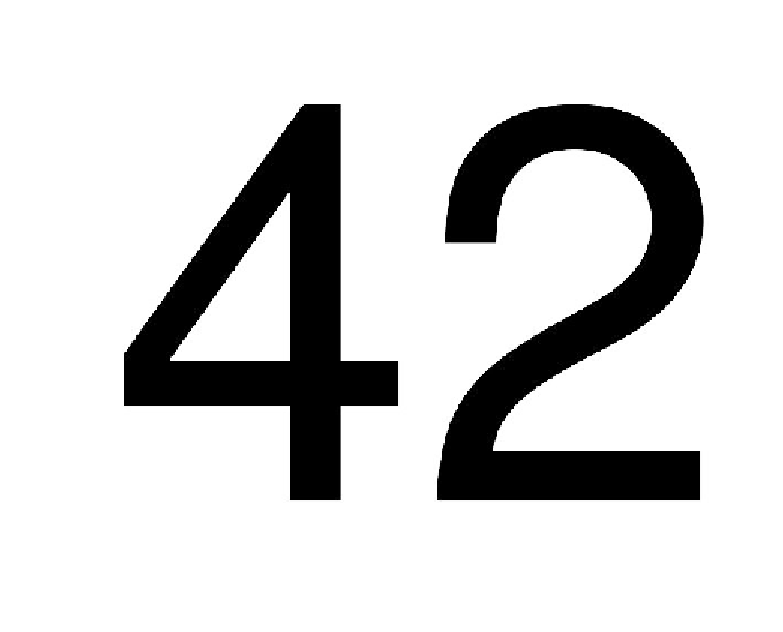
\includegraphics[width=\textwidth]{graphics/svd/42-full.pdf}
        \caption{}
        \label{fig: Theory: SVD-42-full}
    \end{subfigure}
    \hfill
    \begin{subfigure}[b]{0.325\textwidth}
        \centering
        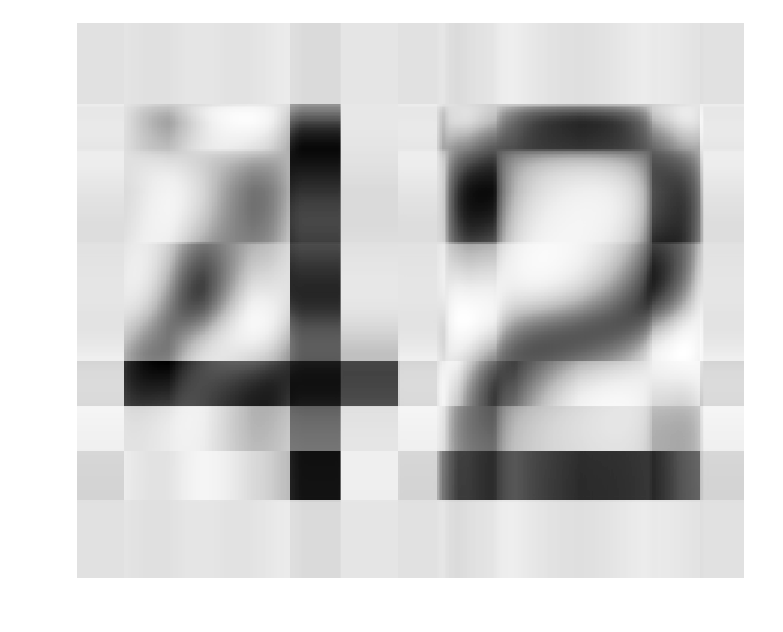
\includegraphics[width=\textwidth]{graphics/svd/42-5.pdf}
        \caption{}
        \label{fig: Theory: SVD-42-5}
    \end{subfigure}
    \hfill
    \begin{subfigure}[b]{0.325\textwidth}
        \centering
        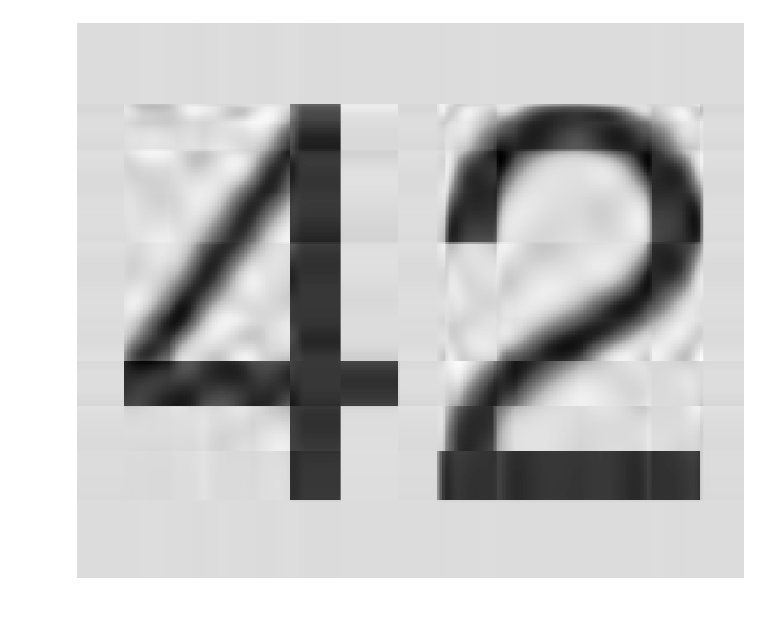
\includegraphics[width=\textwidth]{graphics/svd/42-10.pdf}
        \caption{}
        \label{fig: Theory: SVD-42-10}
    \end{subfigure}
    \caption{
        \subref{fig: Theory: SVD-42-full} An example image of $500\times600=300.000$ pixels.
        \subref{fig: Theory: SVD-42-5} and \subref{fig: Theory: SVD-42-10} Respectively, rank-5 and 10 approximations of the image.
        The low rank approximations are constructed from $5.505$ and $11.010$ parameters, respectively, reduced by a factor of about 56 and 28 compared to the original.
        The high level of structure on the original image results in few large singular values which in turn gives high quality low rank approximations. Note how the axis aligned parts of the ``4" and ``2" are more easily reconstructed.
    }
    \label{fig: Theory: SVD number 42}
\end{figure}
\begin{figure}[tbp!]
    \begin{subfigure}[b]{0.49\textwidth}
        \centering
        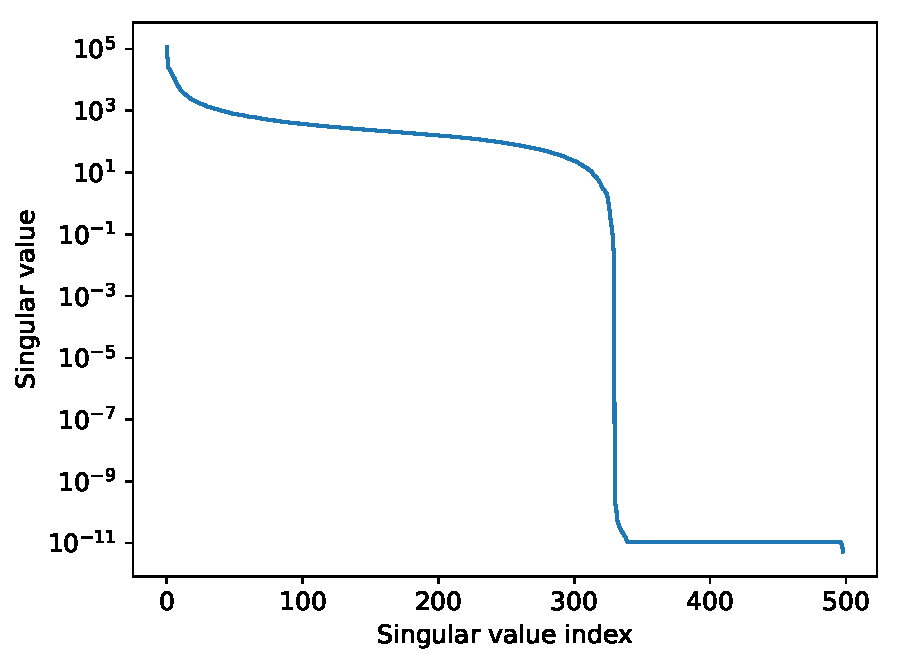
\includegraphics[height=5.7cm]{graphics/svd/42-svds-log.pdf}
        \caption{}
        \label{fig: Theory: SVD-42-svds-log}
    \end{subfigure}
    \hfill
    \begin{subfigure}[b]{0.49\textwidth}
        \centering
        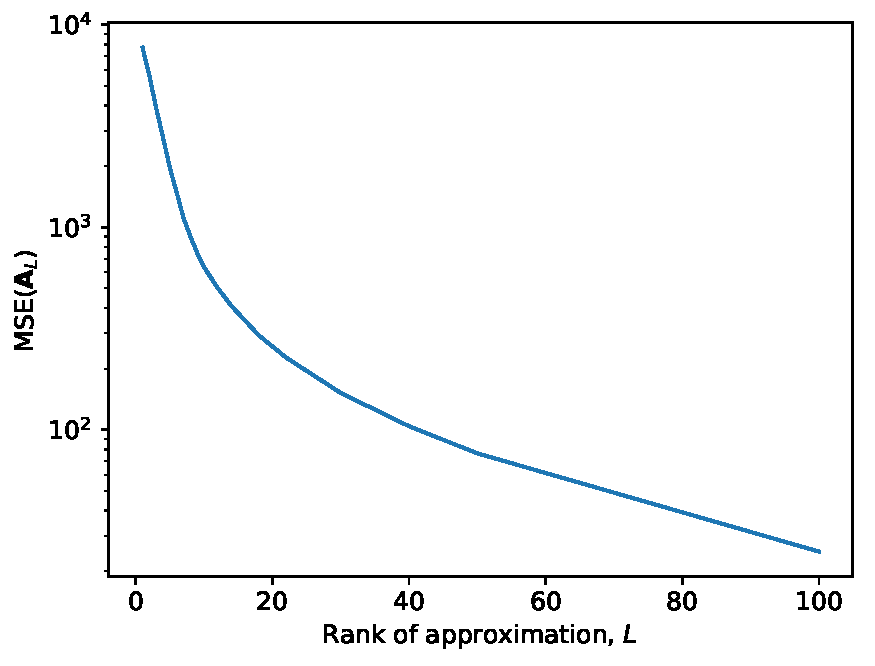
\includegraphics[height=5.7cm]{graphics/svd/42-MSE-log.pdf}
        \caption{}
        \label{fig: Theory: SVD-42-MSE}
    \end{subfigure}
    \caption{
        \subref{fig: Theory: SVD-42-svds-log} Singular values of the image in \autoref{fig: Theory: SVD-42-full} as a function of index.
        \subref{fig: Theory: SVD-42-MSE} \gls{MSE} of different rank approximations of that image.  Note the rapid initial decrease in the singular values driving a steep decrease in the \gls{MSE} over the first $10$ singular values.
    }
    \label{fig: Theory: SVD: singular values and MSE}
\end{figure}

In the context of Gaussian search distributions, the matrix of interest is the covariance matrix which has the additional properties of being symmetric and square and is required to be positive definite. Inspired by the low-rank approximation presented above, a rank-$L$ approximation to the covariance matrix $\Sigmab$ can be written as \cite{Hastie2009}
\begin{equation}
    \Sigmab \approx \D + \sum_{i=1}^L \u_i\u_i\transpose = \D + \U\transpose\U
\end{equation}
where $\u_i$ are $d$ dimensional column vectors and $\U=\bmat{u_1\transpose & \cdots & u_L\transpose}^\text{T}$ has the $\u_i$ vectors in its rows. $\D$ is a diagonal matrix which is chosen large enough that $\Sigmab$ is positive definite. This approximation has $dL$ parameters rather than $d(d+1)/2$ which is considerably fewer for $L\ll d$. 

It seems fair to conjecture that a good approximation might be achievable in this manner for a choice of $L\ll d$ in the case where the search space is the parameter space of an \gls{NN} with $d$ up to hundreds of millions. This thesis has not studied this avenue further.


\subsubsection{Cauchy distribution}
For completeness, this section briefly considers the Cauchy distribution for use in \gls{VO}. Since the Cauchy is a heavy-tailed distribution it can be used for a so-called hill-climber version of \gls{VO} where the population size is 1 \cite{Schaul2011}. 

The \gls{PDF} of the Cauchy is
\begin{equation}
    p(x|\mu,\gamma) = \frac{1}{\pi\gamma}\left[1+\left({\frac{x-\mu}{\gamma}}\right)^{2}\right]^{-1} = \frac{1}{\pi\gamma} \bra{\frac{\gamma ^{2}}{(x-\mu)^{2}+\gamma ^{2}} }
\end{equation}
with log-\gls{PDF}
\begin{equation}
    \log p(x|\mu,\gamma) = - \log(\pi\gamma) - \log\left[1+\left({\frac{x-\mu}{\gamma}}\right)^{2}\right] \ .
\end{equation}
% The gradient of the log-\gls{PDF} is
% \begin{equation}
%     \pderiv{}{x_0}\log p(x|\mu,\gamma) = \frac{2(x-x_0)}{(x-x_0)^2+\gamma^2}
% \end{equation}
% \begin{equation}
%     \pderiv{}{\gamma}\log p(x|\mu,\gamma) = \frac{(x-x_0)^2-\gamma^2}{\gamma\pa{\gamma^2+(x+x_0)^2}} \ .
% \end{equation}
% This is then usable in the \gls{VO} gradient in \eqref{eq: Theory: Variational optimization gradient estimator general search distribution} as the Gaussians. 

At each iteration, a single perturbation is made using the Cauchy and its performance compared to the unperturbed model. If the perturbed model is better it is used as the unperturbed model in the next iteration, otherwise it is disregarded.
Hill-climber \gls{VO} can be better at avoiding getting stuck in local minima. However, due to the rarity of these in the loss surfaces of \glspl{NN} this method is not considered further in this thesis.

%"Making the Cauchy work" introduces the truncated Cauchy which has defined moments \cite{Nadarajah2011}

%\url{https://projecteuclid.org/download/pdfview_1/euclid.bjps/1291387776}

%\todo[inline]{Either write up and include or don't include section on the Cauchy distribution - could be interesting to note Hillclimber version}